\section{The Definite Integral}

For reasons that will not be immediately obvious, integration is opposite differentiation on the `calculus coin.' 

\subsection{The Geometric Definition}

The \textbf{definite integral of $f$ on $(a,b)$} (if such a quantity exists) is the \textit{signed} area between the graph of $f$ and the $x$-axis. 

\begin{figure}[h!]
\label{fig:def-integral}
\centering
\fbox{

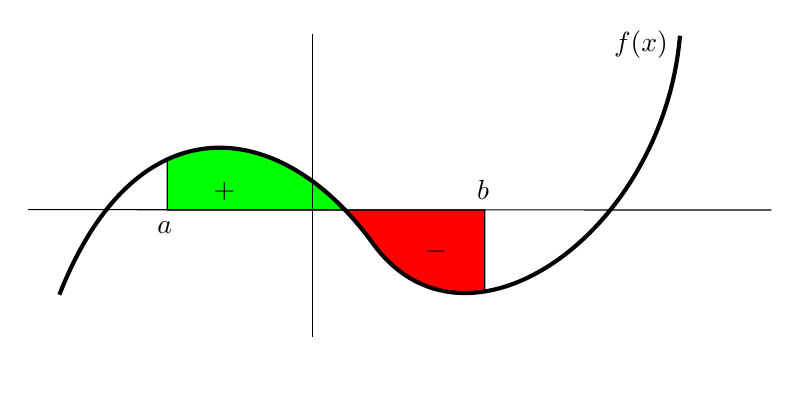
\begin{tikzpicture}[x=0.75pt,y=0.75pt,yscale=-1,xscale=1]
%uncomment if require: \path (0,300); %set diagram left start at 0, and has height of 300

%Shape: Polygon Curved [id:ds707129257032501] 
\draw  [fill={rgb, 255:red, 0; green, 255; blue, 0 }  ,fill opacity=1 ] (217,199) .. controls (217,199) and (217,175) .. (217,175) .. controls (217,175) and (222,171) .. (236,169) .. controls (250,167) and (269,173) .. (278,179) .. controls (287,185) and (288.41,186.01) .. (293,190) .. controls (297.59,193.99) and (302,199) .. (302,199) .. controls (302,199) and (217,199) .. (217,199) -- cycle ;
%Shape: Polygon Curved [id:ds12696670726714787] 
\draw  [fill={rgb, 255:red, 255; green, 0; blue, 0 }  ,fill opacity=1 ] (370,199) .. controls (370,199) and (370,238) .. (370,238) .. controls (370,238) and (355,240) .. (345,237) .. controls (335,234) and (322,224) .. (316,215) .. controls (310,206) and (302,199) .. (302,199) .. controls (302,199) and (370,199) .. (370,199) -- cycle ;
%Straight Lines [id:da2259128899132099] 
\draw    (150,198.8) -- (508,199) ;
%Straight Lines [id:da519801972092973] 
\draw    (287,114) -- (287,260) ;
%Curve Lines [id:da2537963372820191] 
\draw [line width=1.5]    (165,239.8) .. controls (201.6,146.5) and (271,153) .. (316,215) .. controls (361,277) and (456,210) .. (464,115) ;
%Straight Lines [id:da8858936847665124] 
\draw    (217,175) -- (217,199) ;
%Straight Lines [id:da05784827822991523] 
\draw    (370,199) -- (370,238) ;

% Text Node
\draw (211,203.4) node [anchor=north west][inner sep=0.75pt]    {$a$};
% Text Node
\draw (365,183.4) node [anchor=north west][inner sep=0.75pt]    {$b$};
% Text Node
\draw (431,111.4) node [anchor=north west][inner sep=0.75pt]    {$f( x)$};
% Text Node
\draw (238,184.4) node [anchor=north west][inner sep=0.75pt]    {$+$};
% Text Node
\draw (340,213.4) node [anchor=north west][inner sep=0.75pt]    {$-$};


\end{tikzpicture}

}
\caption{The Geometric Definition of the Definite Integral}
\end{figure}


\subsection{Reimann Sums}


\subsection{The Fundamental Theorem of Calculus}


\subsection{Ant-differentiation}


\subsection{Improper integrals}














